% HMC Math dept HW template example
% v0.04 by Eric J. Malm, 10 Mar 2005
\documentclass[12pt,letterpaper,boxed,cm]{hmcpset}

% set 1-inch margins in the document
\usepackage[margin=1in]{geometry}
\usepackage{mathtools}
\usepackage{mathrsfs}
% include this if you want to import graphics files with /includegraphics
\usepackage{graphicx}
\usepackage{cases}
\usepackage{hyperref}
\usepackage{siunitx}
\usepackage{tikz}
\usepackage{cases}
\usetikzlibrary{arrows}

% info for header block in upper right hand corner
\name{Name: ~~~~~~~~~~~~~~~~~~~~~~~~~~~~~~~}
\class{Physics 51}
\assignment{Homework \#13}
\duedate{October 24, 2016}

\newcommand{\ev}[2]{\Big|_{#1}^{#2}}
\newcommand{\evv}[2]{\Big|_{#1}^{#2}}
\newcommand{\set}[1]{\left\{#1\right\}}
\newcommand{\s}[1]{\sqrt{#1}}
\newcommand{\f}[2]{\frac{#1}{#2}}
\newcommand{\p}[2]{\frac{\partial #1}{\partial #2}}
\providecommand{\t}[1]{\text{#1}}
\providecommand{\span}[1]{\text{span}\left(#1\right)}
\providecommand{\set}[1]{\left\{#1\right\}}
\providecommand{\l}[0]{\left}
\providecommand{\r}[0]{\right}
\newcommand{\m}[1]{\begin{matrix}#1\end{matrix}}
\newcommand{\bm}[1]{\begin{bmatrix}#1\end{bmatrix}}
\renewcommand{\bf}[1]{\mathbf{#1}}
\newcommand{\pn}[1]{\left( #1 \right)}
\newcommand{\abs}[1]{\left| #1 \right|}
\newcommand{\bk}[1]{\left[ #1 \right]}
\newcommand{\cis}[1]{\pn{\cos\pn{#1} + i\sin\pn{#1}}}
\newcommand{\cisi}[1]{\pn{\cos\pn{#1} - i\sin\pn{#1}}}
\renewcommand{\Im}[1]{\text{Im}\pn{#1}}
\renewcommand{\Re}[1]{\text{Re}\pn{#1}}
\renewcommand{\k}[0]{\f{1}{4\pi\epsilon_0}}
\renewcommand{\part}[1]{\vspace{1em}\noindent(#1)}

\makeatletter
\renewcommand*\env@matrix[1][*\c@MaxMatrixCols c]{%
  \hskip -\arraycolsep
  \let\@ifnextchar\new@ifnextchar
  \array{#1}}
\makeatother
\begin{document}
\problemlist{33-P13*, 34-E23, 34-E30, 34-P9}


\begin{problem}[33-P13*]
The current density inside a long, solid, cylindrical wire of radius $a$ is in the direction of the axis and varies linearly with radial distance $r$ from the axis according to $j = j_0r/a$. Find the magnetic field inside the wire. Express your answer in terms of the total current $i$ carried by the wire.	
\end{problem}
\begin{solution}
\end{solution}
\newpage


\begin{problem}[34-E23]
A rectangular loop of wire with length $a$, width $b$, and resistance $R$ is placed near an infinitely long wire carrying current $i$, as shown in Fig. 34-49. The distance from the long wire to the loop is $D$. Find
\begin{enumerate}
	\item[(a)] the magnitude of the magnetic flux through the loop and 
	\item[(b)] the current in the loop as it moves away from the long wire with speed $v$.
\end{enumerate}
\begin{center}
	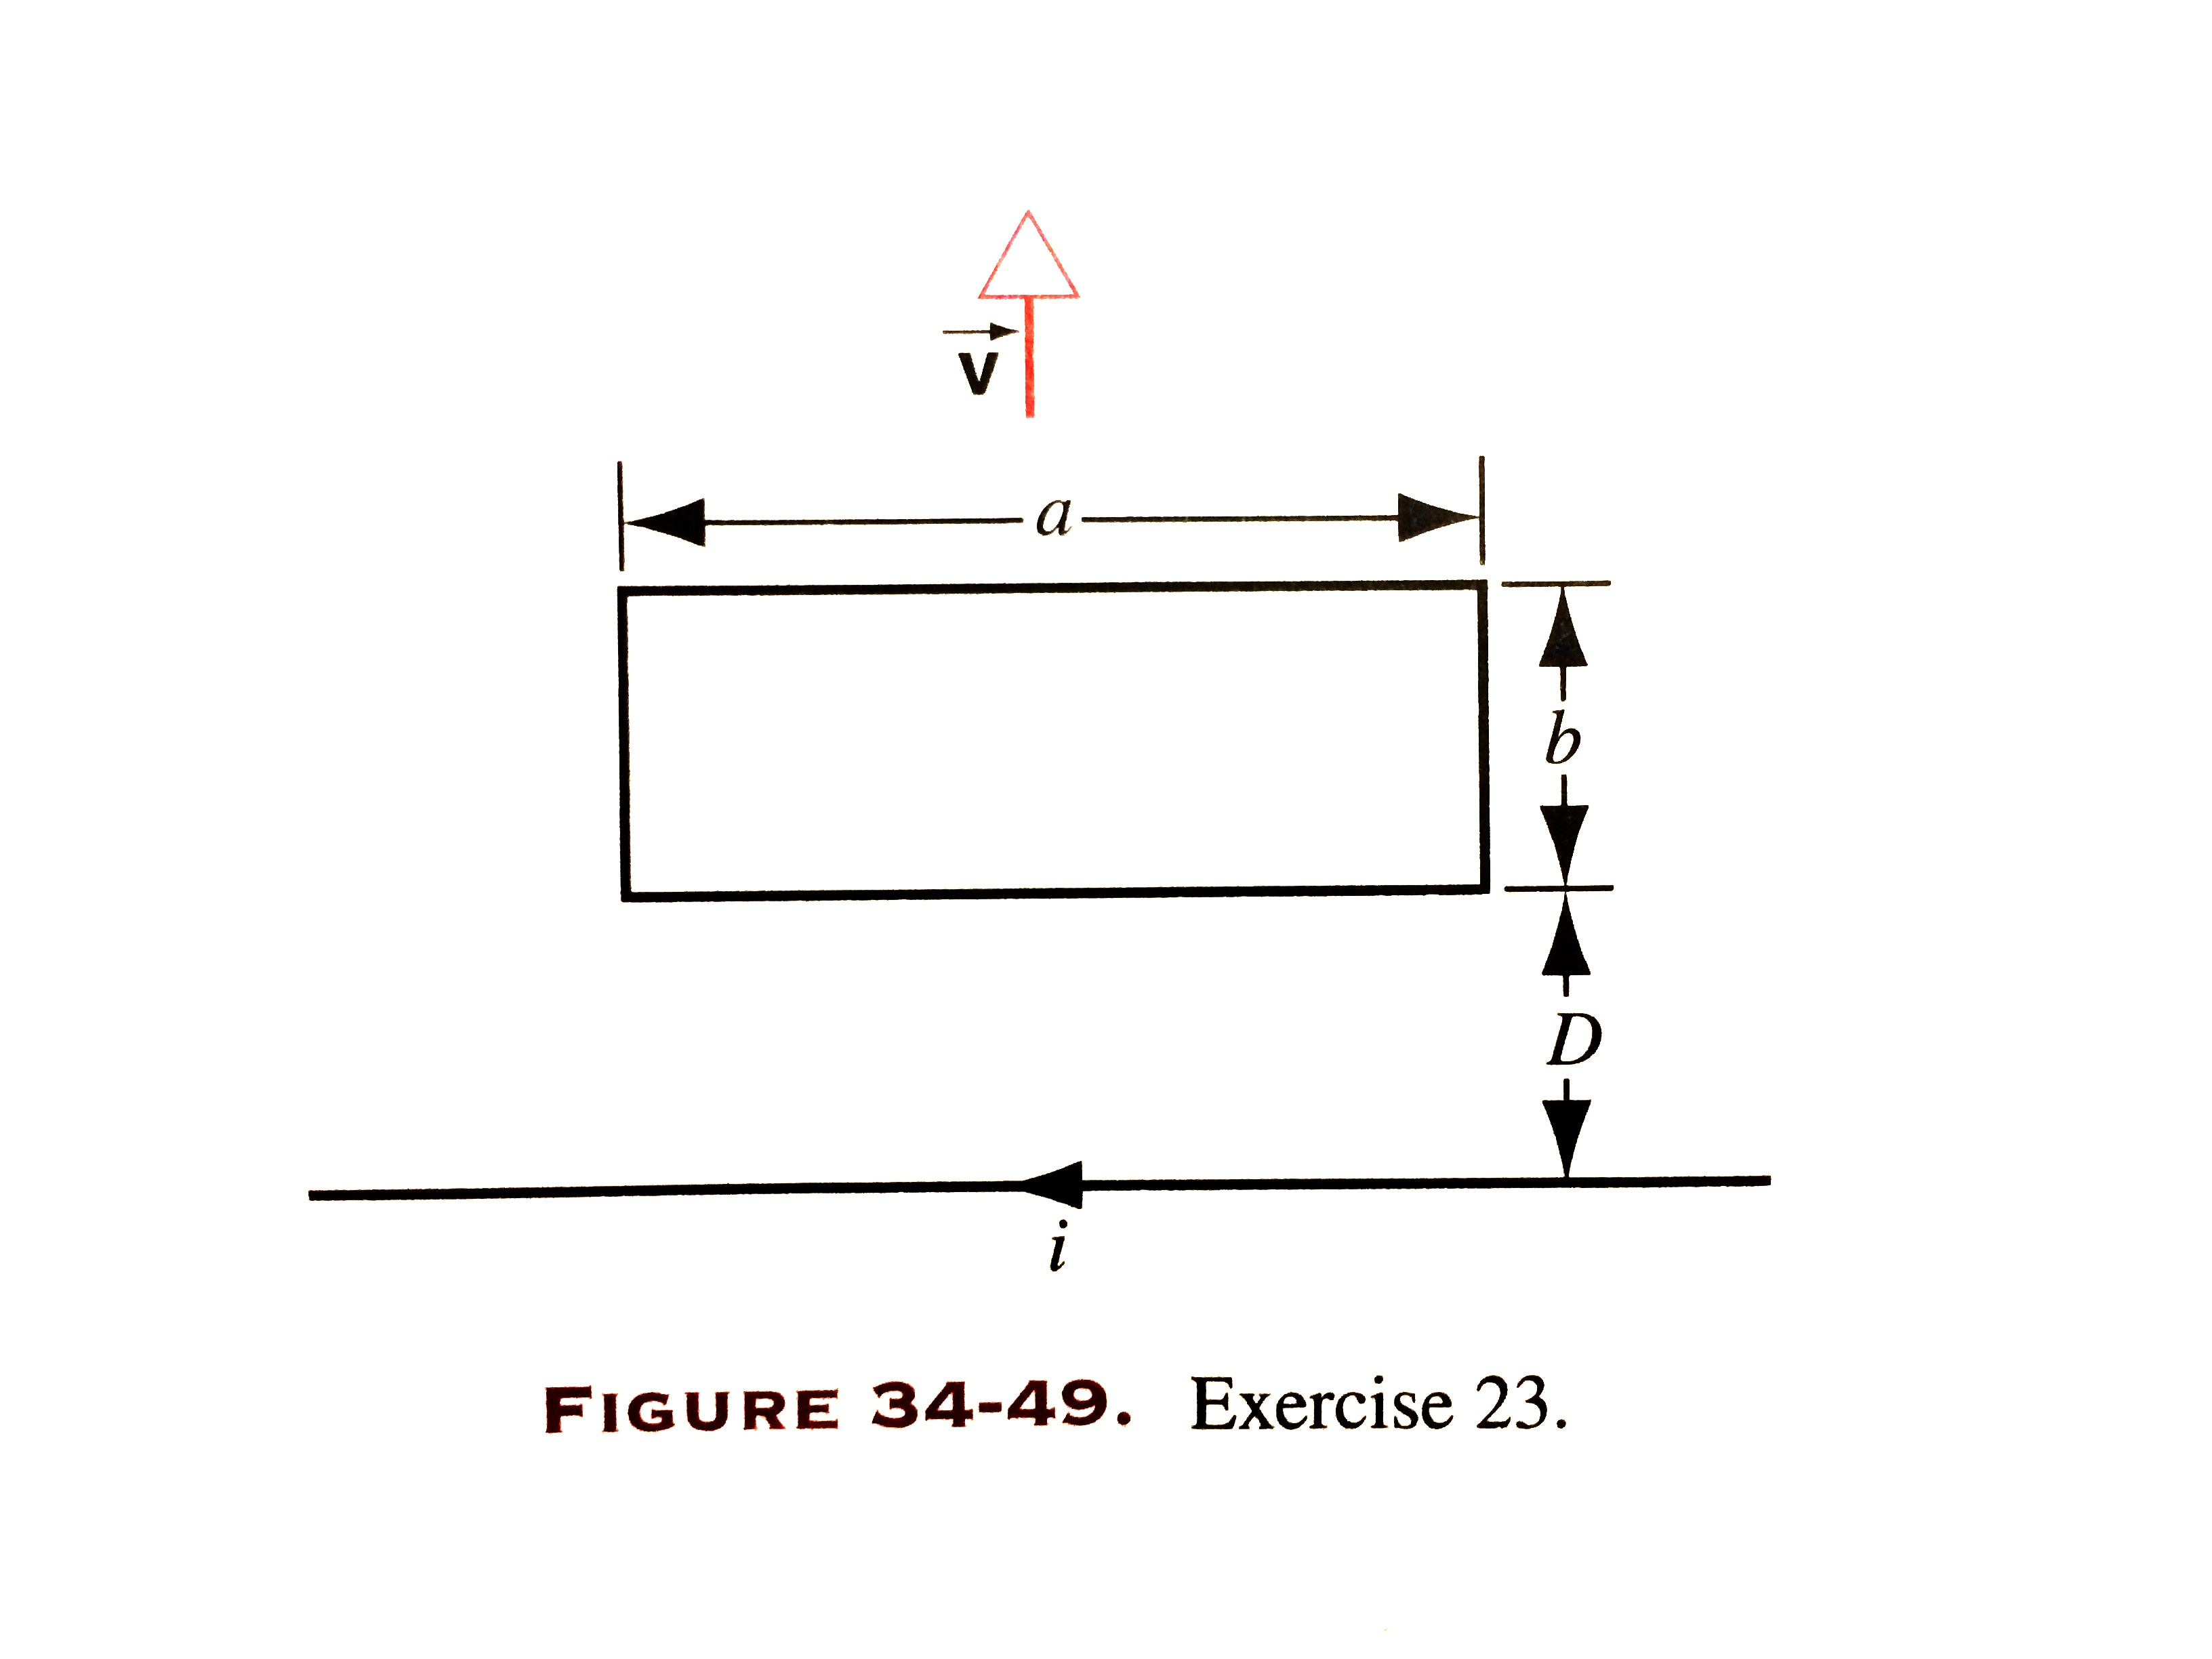
\includegraphics[scale=0.1]{01.jpeg}	
\end{center}
\end{problem}
\begin{solution}
\end{solution}
\newpage

\begin{problem}[34-E30]
A long solenoid has a diameter of $\SI{12.6}{cm}$. When a current $i$ is passed through its windings, a uniform magnetic field $B = \SI{28.6}{mT}$ is produced in its interior. By decreasing $i$, the field is caused to decrease at the rate $\SI{6.51}{mT/s}$. Calculate the magnitude of the induced electric field
\begin{enumerate}
	\item[(a)] $\SI{2.20}{cm}$ and
	\item[(b)] $\SI{8.20}{cm}$ from the axis of the solenoid.
\end{enumerate}
\end{problem}
\begin{solution}	
\end{solution}
\newpage

\begin{problem}[34-P9]
	A rod with length $L$, mass $m$, and resistance $R$ slides without friction down parallel conducting rails of negligible resistance, as in Fig. 34-59. The rails are connected together at the bottom as shown, forming a conducting loop with the rod as the top member. The plane of the rails makes an angle $\theta$ with the horizontal, and a uniform vertical magnetic field $\vec{\mathbf{B}}$ exists throughout the region.
	\begin{enumerate}
		\item[(a)] Show that the rod acquires a steady-state terminal velocity whose magnitude is
		\[
			v = \f{mgR}{B^2L^2} \f{\sin\theta}{\cos^2\theta}.
		\] 
		\item[(b)] Show that the rate at which the internal energy of the rod is increasing is equal to the rate at which the rod is losing gravitational potential energy.
		\item[(c)] Discuss the situation if $\vec{\mathbf{B}}$ were directed down instead of up.
	\end{enumerate}
	\begin{center}
		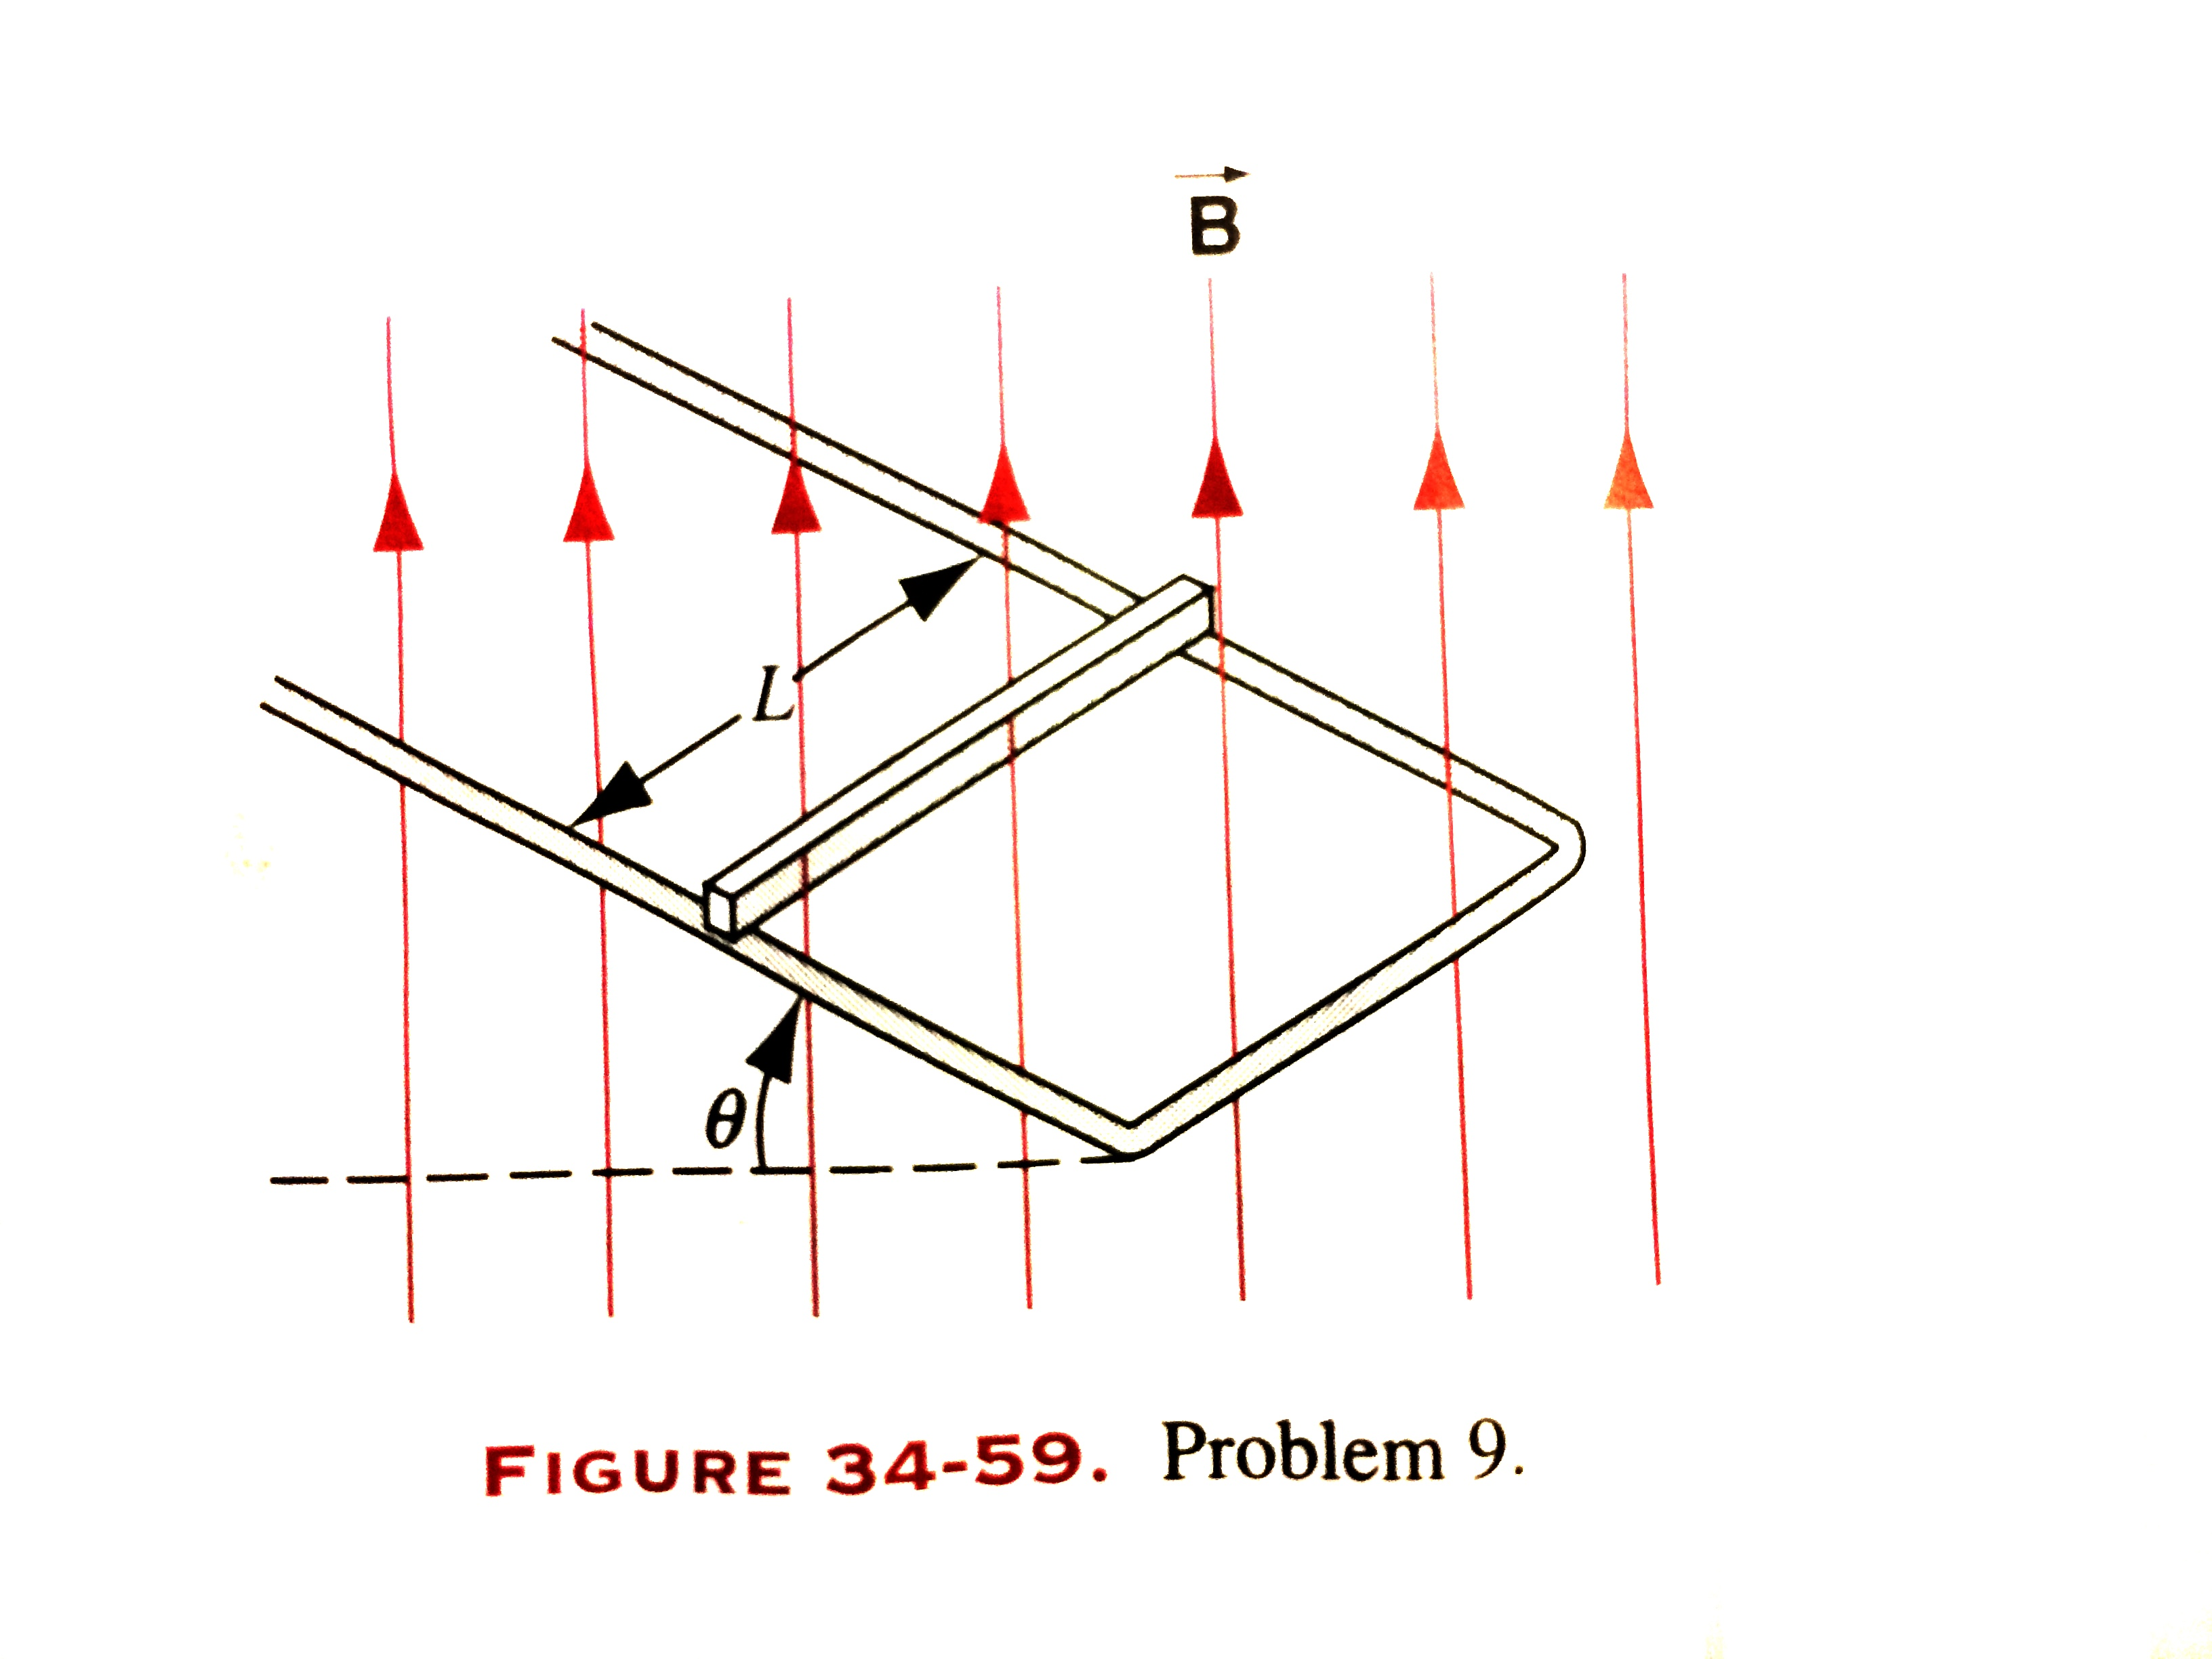
\includegraphics[scale=0.1]{02.jpeg}
	\end{center}
\end{problem}
\begin{solution}
\end{solution}

\end{document}